\documentclass[12pt]{report}

\usepackage{graphicx}
\usepackage{textcomp}
\usepackage[margin=1.0in]{geometry}
\usepackage[symbol]{footmisc} % Used to have symbols for footnotes instead of numbers (so as to not get confused between references and footnotes)
\usepackage{gensymb} % Used for the degree symbol in math mode
\usepackage[subrefformat=parens,labelformat=parens]{subfig} % Used to combine figures into one
\usepackage{cleveref} % Makes references easier
\usepackage{bm} % Used for bold font in math mode
\usepackage[superscript,biblabel,sort]{cite} % The superscript option puts the references as superscript numbers, biblabel applies the superscript to the references page, and sort sorts the numbers from least to greatest, and if possible, puts a dash to shorten it (i.e. 1,2,3,4,5,6 will be shortened to 1-6)

\bibliographystyle{aip2}

% This is the Introduction and Background section of the paper
\begin{document}
\chapter{Introduction}

Nuclear energy has long been of interest to the world as a possible source of energy.  Despite the promise of a long-term solution to the renewable-energy problem, fears still grip the hearts of civilians and government officials across the world because of bombs such as the ones used on Japan during World War II, and because of nuclear reactor catastrophes such as Three Mile Island, Chernobyl, and most recently Fukushima.  A major part of addressing these fears is making the operation of nuclear reactors more safe.  Part of the concern with nuclear energy is the radioactivity associated with nuclear materials, so minimal exposure to the material is sought after.  ``Minimal exposure" in part means that nuclear fuel should be used as efficiently as possible, reducing the need to refuel and limiting radiation exposure to human and machine alike.  Nuclear fuels have been and continue to be extensively studied to achieve the safety and efficiency sought after with this major energy source.

% Nuclear reactors have many variables that need to be taken into consideration
% 1) Quality of the fuel.
% 2) Understanding of the fuel's material properties
% 3) Understanding how the reactor itself will respond to radiation
% 3) Operating conditions
% 4) Emergency procedures

In order for a nuclear reactor to work properly, many things need to be taken into consideration.  First, understanding the ideal operating conditions for the nuclear reactor is important so immediate actions can be taken when conditions are no longer ideal.  Radioactivity has an effect on all materials, not just living tissue.  Over time, radiation can create defects in the crystal structures of the metals used to create the reactor shell, and these defects can build up, causing deformation, weakening, or stiffening of the materials, which can lead to problems if not properly managed.\cite{callister2003}.  As the reactions continue, more neutrons are created potentially causing additional fission events.  In order to prevent the reactor from having all the fissile material fission at nearly the same time (releasing a large amount of energy), various methods are in place controlling the number of chain reactions.  Emergency procedures also are in place to prevent catastrophes as mentioned above.

Second, the quality of the fuel must meet a minimum standard in order for a sustainable reaction to occur.  Nuclear fuels are divided into two categories: fissile (where bombardment of the material with neutrons will divide the atomic nuclei into ``daughter" particles, releasing energy), and non-fissile (bombardment of the material results in the neutrons becoming part of the nucleus, called absorption).  Fissile materials are required for nuclear reactors to work.  One of the most common fissile materials used is an isotope of uranium called U-235.  A second isotope of uranium, U-238, is much more common in the earth (approximately 99\% of all uranium).  In order to have a sustainable chain-reaction, the amount of U-235 present in a fuel pellet must be at a certain level, depending on the moderating medium.\cite{uraniumInfo}

Third, the various properties of the fuel need to be well understood in order to make the running of the reactor as safe and effective as possible.  Some of these properties include the thermal conductivity (how well heat flows through the material), the fission gas release (how some of the fission products move throughout the material as gases), and the mechanical stability (i.e. how the material bends or cracks under pressure or heat).  Taking the thermal conductivity as an example, knowledge of this material property allows the coolant to be used most effectively to keep the reactor within operating temperatures, maximizing both efficiency and safety.  Knowledge of other material properties allows for similar gains in efficiency, safety, or both.

Uranium dioxide (UO\textsubscript{2}) is the primary choice for nuclear fuel in today's reactors.\cite{uraniumInfo}  In order to understand the properties of UO\textsubscript{2} as described above, an analysis of the basic crystal structure of the material is required.  UO\textsubscript{2} is a ceramic, and as such is made up of a series of crystal lattices joined together in various ways.  This material has a fluorite crystal structure, meaning that the uranium atoms form a face-centered cubic (fcc) lattice, and the oxygen atoms form a simple cubic lattice within the fcc frame (see \Cref{fig:uo2Lattice}).  This work adds to the safety and efficiency of using nuclear energy by providing the necessary information to accurately calculate the material properties of UO\textsubscript{2} in-reactor.

\begin{figure}[ht!]
\centering
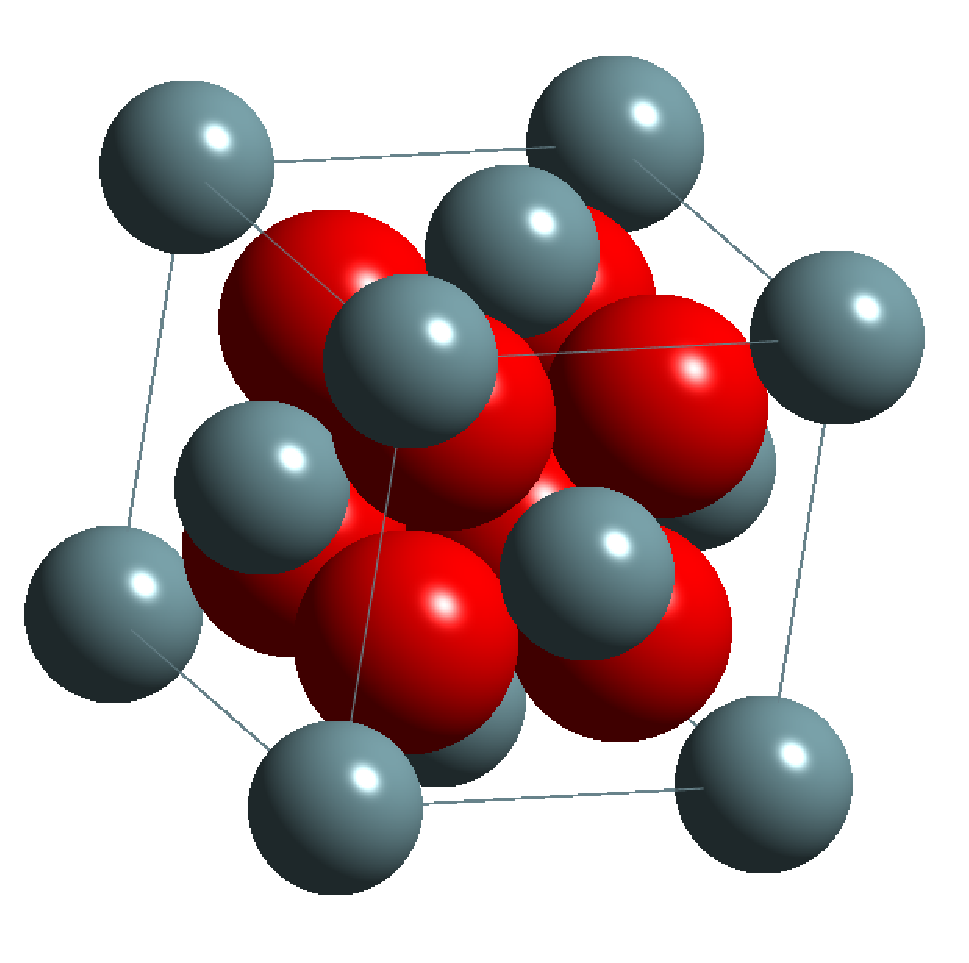
\includegraphics[scale=1.0]{Images/UO2}
\caption{\label{fig:uo2Lattice}An image representing the fluorite crystal structure.  For UO\textsubscript{2}, the gray spheres indicate the uranium atoms, and the red spheres indicate the oxygen atoms.  Image courtesy of the University of Cambridge under the Creative Commons license.}
\end{figure}

\section{Background}
Ceramics, metals, and polymers are composed of tiny groups of crystals called \emph{grains}.  The orientation of each grain is generally independent of the orientation in the grains surrounding it meaning there is a possibility (depending on how the crystal was formed\cite{callister2003}) that crystal structures will not line up at the interfaces where these two grains meet.  This mismatch leads to broken or stretched atomic bonds where atoms will not be in the right place relative to a perfect crystal structure.  These defects are called grain boundaries (GBs), and an example of a GB can be seen in \Cref{fig:gb}.  At the GB there is an ``atomic mismatch"\cite{callister2003} where individual atoms are shifted relative to the exact crystal structure provided by the bulk of the grain.  The most popular way to parameterize a GB is to use the five degree of freedom (DoF) model.\cite{patala2013, lejcek2010, homer2015, bulatov2014, harbison2015, rohrer2011}.  This model only uses the macroscopic DoFs, ignoring the three translational DoFs possessed by each grain.  Three of the five DoFs specify the misorientation of the grains with respect to each other.  The other two DoFs specify the orientation of the grain boundary plane (called the inclination).  The misorientation DoFs are the rotation angle $\theta$ (one of three) and the rotation axis (another two angles), while the inclination DoFs are defined by the normal of the grain boundary (two angles).\cite{lejcek2010}

There are three specific types of GBs that polycrystalline materials have: twist, tilt, and mixed GBs.\cite{lejcek2010, rohrer2011}  These GBs desribe the misorientation of two grains with respect to each other.  A twist boundary is when the axis of rotation between the two grains is parallel to the GB normal.  Tilt boundaries are composed of symmetric tilt and asymmetric tilt boundaries.  A tilt boundary occurs when the axis of rotation between the two grains is perpendicular to the GB normal.  Symmetric tilt boundaries occur when the boundary plane is a mirror plane: one side of the boundary is the mirror of the other.  Thus, the angles between the boundary plane and the grains are equal. Asymmetric tilt is when the angles are not equal.  \Cref{fig:misorientation} shows a representation of tilt boundaries (top) and twist boundaries (bottom).  A mixed GB is a combination of twist and tilt boundaries in some degree.

Understanding GBs is important because of the differing effects they have on material properties.\cite{patala2013, homer2015, bulatov2014}  Part of this understanding comes from knowing how the GBs will evolve in time.  Because of the atomic mismatch at the boundaries extra energy is in the crystal structure.  This extra energy (called GB energy) gives rise to grain boundary motion.  Thus, in order to accurately model how GBs evolve and how the material properties change, the GB energy needs to be fully understood.

There are two ways to approach GB energy.  The most common method (and easier method) is to assume an isotropic model.  This model ignores the impact of inclination on the GB energy, and assumes that all inclinations for a given misorientation are equal, reducing the 5D parameter space to a 3D parameter space.  The reasons for assuming this model historically have been because it was assumed that the inclination had little or no impact on the GB energy, or (later) that it was too difficult to create a full five DoF model.\cite{homer2015}

Alternatively, there is the anisotropic approach.  This approach seeks to quantify the effect that inclination has on the GB energy.  Currently researchers have acknowledged the need for a full five DoF model for the GB energy, but have asserted the difficulty inherent in developing such a model.\cite{rohrer2011, lejcek2010, homer2015}  There is not yet a universal function to describe GB energy anisotropy in every crystalline material, but some researchers\cite{bulatov2014} have created successful models for a subset of materials.

%\begin{figure}[ht!]
%\centering
%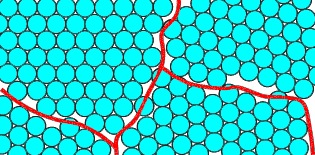
\includegraphics[scale=1.0]{Images/grainBoundary}
%\caption{\label{fig:gb}An example of a grain boundary.  Individual atoms of the grains are the blue circles, while the grain boundary is highlighted by the red line.  Atomic mismatch between the differently oriented grains causes an excess of energy to be present within the material, which has an effect on the material's properties.  Image courtesy of the University of Cambridge under the Creative Commons license.}
%\end{figure}

%\begin{figure}[ht!]
%\centering
%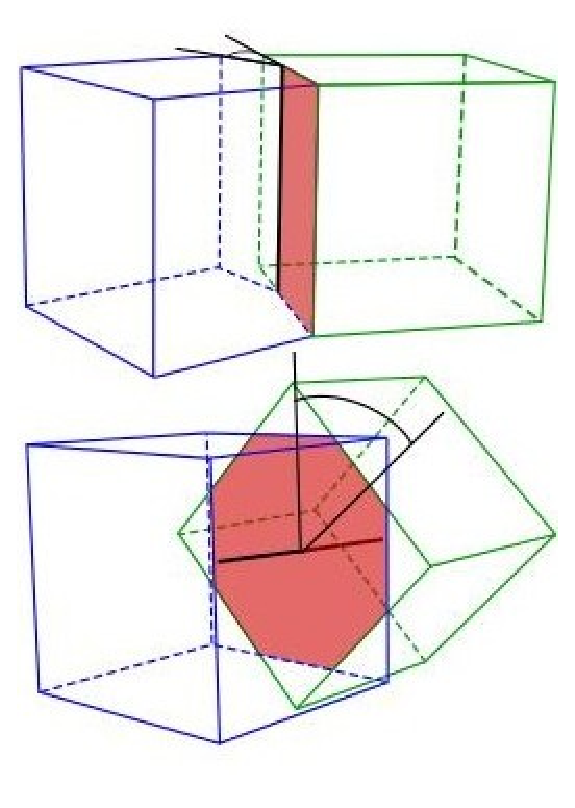
\includegraphics[scale=1]{Images/twistTilt}
%\caption{\label{fig:misorientation} An example of a tilt GB (top) and a twist GB (bottom).  The axis of rotation for the tilt GB is perpendicular to the GB normal, and for the twist GB is parallel to the GB normal.  Image courtesy of Wikipedia under the Creative Commons license.}
%\end{figure}

\begin{figure}[ht!]
 \centering
 
 \subfloat[]{\label{fig:gb}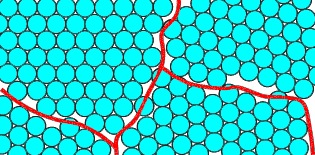
\includegraphics[scale=.9]{Images/grainBoundary}}\quad
 \subfloat[]{\label{fig:misorientation}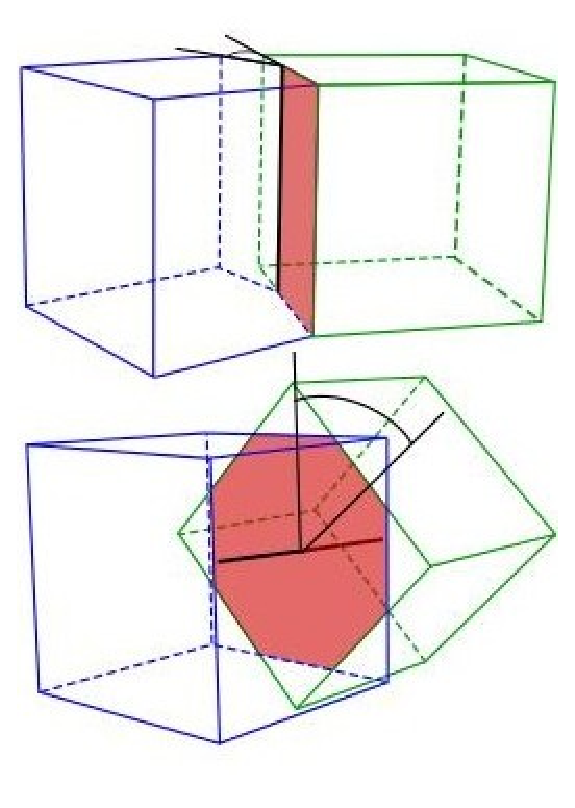
\includegraphics[scale=.6]{Images/twistTilt}}\quad
 \caption{\label{gbs} A representation of GBs, where \protect\subref{fig:gb} shows an example of a grain boundary and \protect\subref{fig:misorientation} shows an example of GB types.  In \protect\subref{fig:gb} individual atoms of the grains are the blue circles, while the grain boundary is highlighted by the red line.  Atomic mismatch between the differently oriented grains causes an excess of energy to be present within the material, which has an effect on the material's properties.  Image courtesy of the University of Cambridge under the Creative Commons license. In \protect\subref{fig:misorientation} the axis of rotation for the tilt GB (top) is perpendicular to the GB normal, and for the twist GB (bottom) is parallel to the GB normal.  Image courtesy of Wikipedia under the Creative Commons license.}
\end{figure}

\section{Previous Work}
Bulatov \emph{et al.}\cite{bulatov2014} developed a five DoF function which accurately interpolates any arbitrary GB energy for fcc metals.  They used energies for GBs along specific axes to interpolate the full 5D space.  A more detailed explanation of their methods is presented in the methods section of this paper.  Harbison\cite{harbison2015} applied the same ideas towards developing a five DoF function which interpolates any arbitrary GB energy in UO\textsubscript{2}.  GB energies were gathered for various misorientations around a high-symmetry axis using molecular dynamics (MD) simulation results.  The fitting procedure created a set of 43 parameters defining the function needed to interpolate an arbitrary GB energy.

This work improves the fitting parameters by using MD results calculated with an anneal of 800K.  Harbison's work did not anneal the crystal structure\cite{harbison2015}, which prevented the atoms from finding their ideal energetic minimum.  The 800 K anneal allows the atoms to relax to a value closer to their global minimum, as will be shown in the results.  The energies from these simulations will be incorporated into a database that a MATLAB\textsuperscript{\textregistered} script will use to fit the function parameters.  The updated parameters will be incorporated in Idaho National Laboratory's (INL's) mesoscale phase field modeling platform MARMOT for use in modeling nuclear fuels.  As these parameters are implemented in the modeling software, various tests of the UO\textsubscript{2} fuel can be performed to determine how the material properties change while in-reactor. 

\bibliography{gbCharacter}
\end{document}